
\clearpage
\section{Import}

\begin{wrapfigure}[3]{l}{6.5cm}   % [x] Wie manche Zeile soll sich um die Grafik "brechen"
  \vspace{-35pt}      % Grundwert war 20; mit 30 schön oben beim Text ausgerichtet
  \begin{center}
    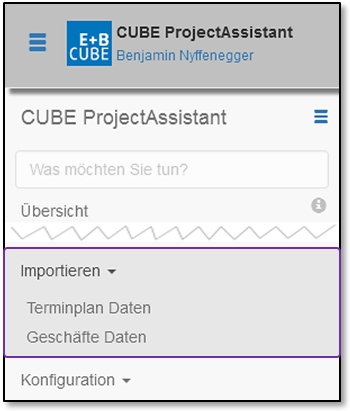
\includegraphics[width=1\linewidth]{../chapters/12_Importieren/pictures/12_Menu_Importieren.jpg}
  \end{center}
  \vspace{-20pt}
  \caption{Importing data}
  \vspace{-10pt}
\end{wrapfigure}

In the menu on the left select the 'Import' menu item and the the desired subcategory: 'Project plan data' or 'Transaction data'.
\vspace{6.5cm}

\subsection{Project Plan Data}
\label{bkm:Ref445411998}

\begin{wrapfigure}[10]{r}{6cm}
\vspace{-15pt}
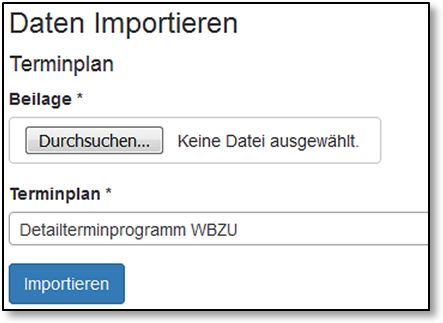
\includegraphics[height=50mm]{121_DatenImportieren.jpg}
\caption{Importing data}
\end{wrapfigure}
Using the 'Project Plan Data' import function, a new, up-to-date detailed scheduling program can be imported. The project planning is carried out in Microsoft Project and exported as a XML file then imported into CUBE PA. By doing so, the existing data in CUBE PA is lost. The imported data cannot be edited, but only viewed. It is also possible to view the project planning and to zoom in on the desired time window on computers without Microsoft Project. Further information can be found in chapter \ref{bkm:Ref445400921} 'Scheduling'.

\vspace{\baselineskip}

In order to use the additional view and filter options (project / subproject / resources) in CUBE PA, the MS Project file must already contain the corresponding information. The resources are defined beforehand according to the usual MS Project procedures and then assigned to the individual processes. The assignment of the processes to a project / subproject is possible with the help of user-defined fields. To do so, two new columns should be added to the Project file (text type, e.g. Text1 and Text2). These columns should be named 'Subproject\_1' and 'Subproject\_2' in the Gantt chart view \col{(1)}, either directly in the table or under Format, User-defined fields. This enables the correct importing of data into CUBE PA. The individual processes can then be assigned to the projects (subprojects) according to the tag definitions in CUBE PA. To do so, the project names can be entered manually or using the drop-down menu in the columns 'Subproject\_1' and 'Subproject\_2'. Before the export/import, it must be checked that all processes are assigned to the correct projects and that no fields are left empty. This is the only way to prevent processes from being mistakenly hidden by the later filtering in CUBE PA.

\begin{figure}[H]
\center{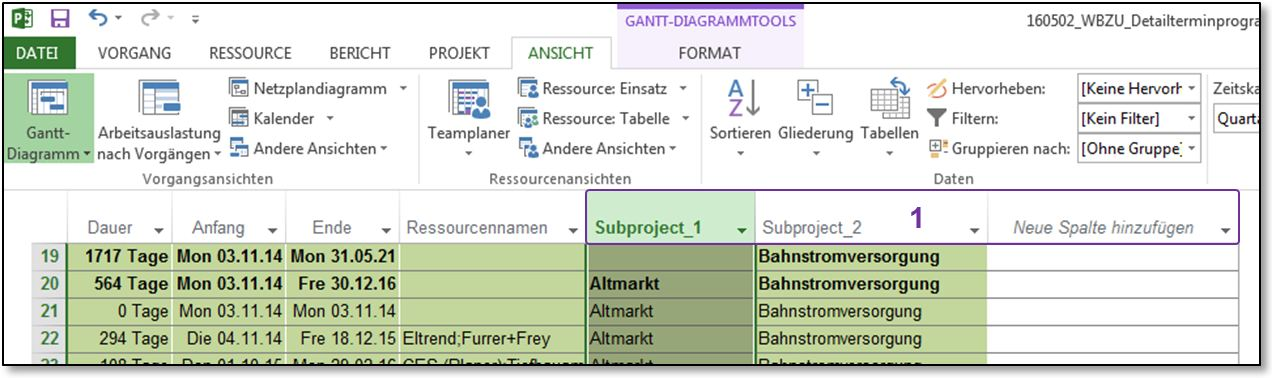
\includegraphics[width=1\linewidth]{121_zusSpaltenMSProject.jpg}}
\caption{Additionally required columns in MS Project}
% \label{fig:speciation}
\end{figure}

\subsection{Transaction Data}

Follows later.
